%% This section adds chapter 4
\section{Background}

A key component of contemporary software development is now \ac{oss}. Software that is freely accessible for use, alteration, and dissemination is referred to. Because of its collaborative development philosophy and advantages for both users and developers, the open-source movement has grown significantly in popularity in recent years.

\subsection{Origins and Early Practices}

Open source software has its roots in the early years of computers, when cooperation and sharing were common practices. Code was openly shared and altered by programmers in academic environments, motivated by a desire to enhance the technology they utilized. However, as software began to be commercialized, this openness clashed with the rise of proprietary software models. Restrictions on use and a lack of transparency led to frustration among many programmers, sparking the desire for an alternative.

In 1983, Richard Stallman's launch of the GNU Project became a catalyst for the modern open source movement \cite{dibona1999open}.  This ambitious initiative aimed to create a completely free operating system built on the principles of software freedom.  Stallman's advocacy for free redistribution, user modification rights, and transparent development laid the philosophical foundation for the open source movement.

Early open source projects relied heavily on collaborative development through online communities of programmers. This distributed model allowed for efficient bug fixing, rapid development, and fostered knowledge exchange.  Moreover, the creation of licenses like the GNU \ac{gpl} was crucial. These licenses protected open source freedoms, ensuring that software and any modifications made to it would remain accessible to all \cite{license1989gnu}.


Several notable projects defined the early era of open source software. Linus Torvalds' creation of the Linux kernel in 1991 became the poster child for successful open source development, eventually forming the heart of countless operating systems. Additionally, the GNU Project provided essential tools, the Apache Web Server became the dominant force powering the internet, and BIND played a critical role in the internet's infrastructure. These landmark projects proved the viability and potential of the open source model.


\subsection{Defining Open Source}
There is debate about what define open source software. It sparks debate between those who see it as synonymous with "free software" and those who view "open source" as a distinct approach \cite{FuggettaAlfonso2003Osse}.

"Free software", a term stemming from the GNU project, prioritizes user freedoms over cost. At its core, free software grants users the right to use, share, study, modify, and even improve software without restrictions \cite{Whatisfreesoftware}.  Access to the source code is vital, as it is what empowers users to exercise these freedoms.

The term "open source" was introduced later than "free software." While both aim to describe software with accessible source code, there are key philosophical differences. The "open source" term was partly motivated by a desire for a less politically charged, business-friendly label, though its official definition aligns closely with "free software". Stallman argues that the everyday interpretation of "open source" merely denotes visibility of the source code, not the full freedoms of free software \cite{StallmanWhyOpenSource}. This ambiguity allows the term to be applied to semi-free or even proprietary software, diluting its meaning.


Open source projects come in a variety of shapes and sizes, there are two primary types: open source software and open source content \cite{OregShaul2008Emfc}. Code that is openly accessible for anyone to view, alter, and distribute is referred to as open source software. This cooperative strategy encourages creativity and quick progress. On the other side, open source content includes a greater variety of creative elements, including artistic creations, scientific data, and educational tools. Similar to software, licensing for open source content allow users to access, distribute, and alter the information within certain bounds.

\subsection{Open Source Project}
An open-source project is a cooperative effort in which the public is given unrestricted access to the source code of a software program or application. This indicates that, in accordance with the conditions of the project's license, anybody may access, alter, and distribute the code. Open-source initiatives frequently promote openness, community-driven development, and cross-disciplinary developer cooperation.

One of the most common used definitions of open source comes from the Open Source Initiative (OSI), which defines open source software as having a license that meets the following criteria in the figure \ref{fig:osidef}.

\begin{figure}[ht]
    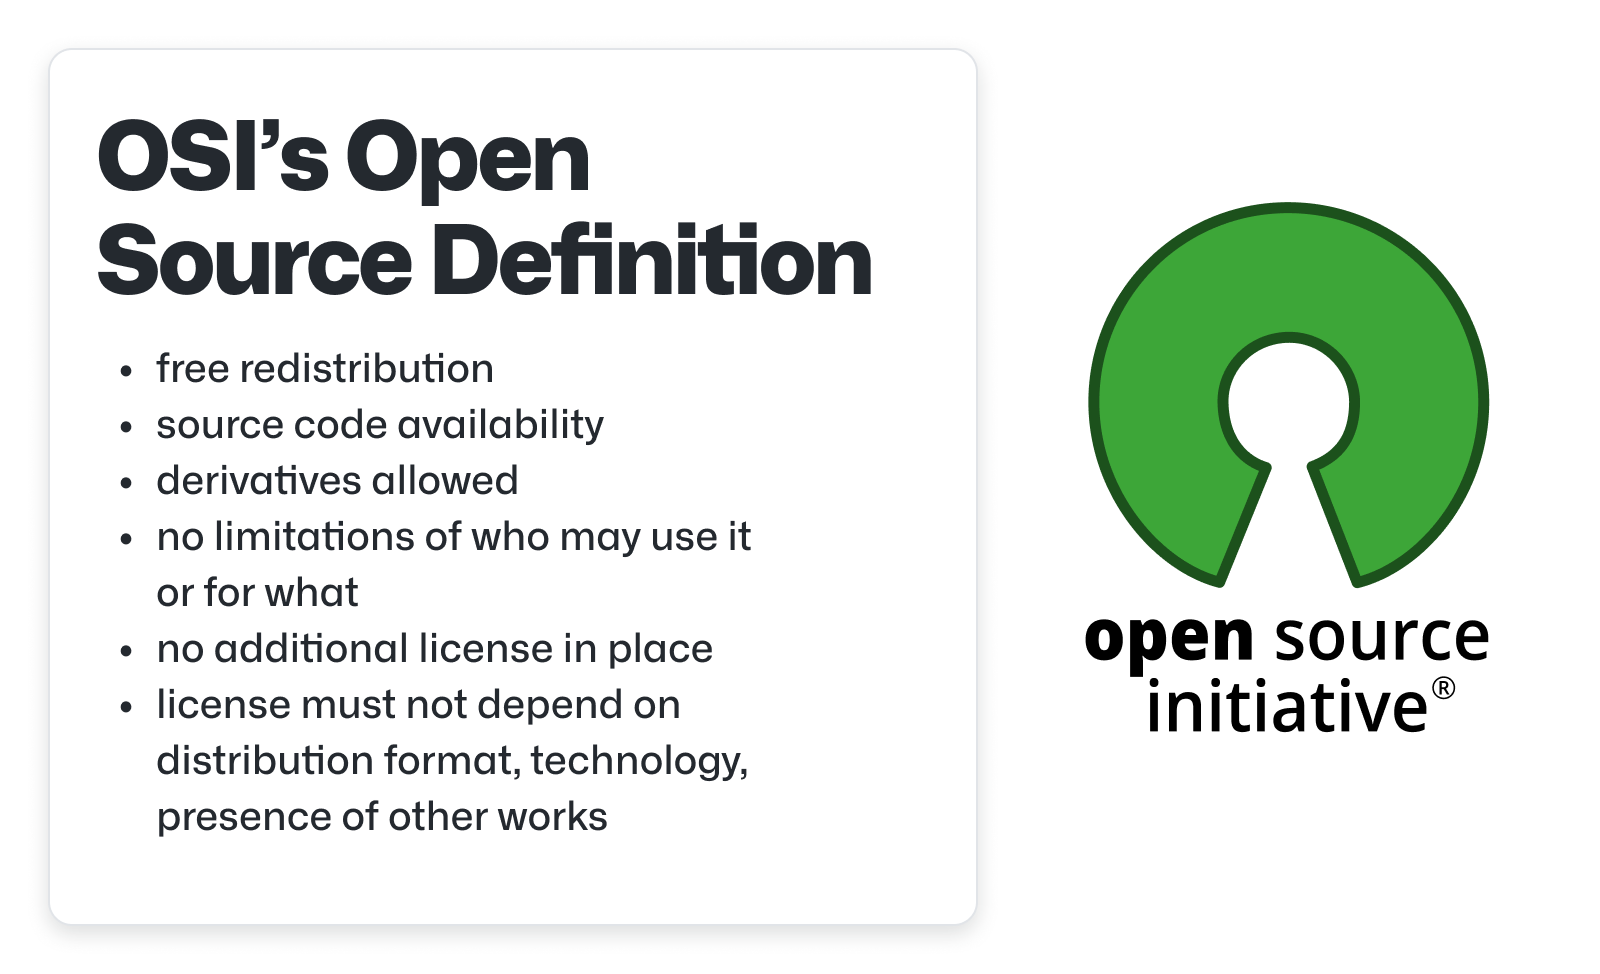
\includegraphics[width=12cm]{figs/osiopensourcedef.png}
    \centering
    \caption{OSI's Open Source Definition \cite{HaeussgeDevGuide}}
    \label{fig:osidef}
\end{figure}



Among the most well-known and significant OSS projects are:
\begin{itemize}
    \item Linux: A very well-liked and adaptable kernel for operating systems. Numerous gadgets, including smartphones, embedded systems, servers, and supercomputers, are powered by Linux. It is renowned for its security, stability, and customizability \cite{fink2003business}.
    \item Git: A widely-used system that helps developers manage and track changes to their code. It has become the preferred tool in software development, enabling collaboration and allowing developers to explore different versions of their project without affecting the main codebase \cite{loeliger2012version}.
    \item Apache HTTP Server: A very popular software used to deliver web content. It powers a large number of websites and is known for being dependable, adaptable, and feature-rich \cite{fielding1997apache}.
    \item  Python: A user-friendly programming language designed for clarity and simplicity. It is widely used in various fields such as data science, web development, machine learning, and system administration. \cite{srinath2017python}.
    \item TensorFlow: A free, open-source framework designed to make machine learning accessible. It offers a wide range of tools, libraries, and a supportive community, so both researchers and developers can create and use powerful ML applications \cite{developers2022tensorflow}.
\end{itemize}

\subsection{Ownership and Licensing}

The concept of ownership within the open-source software landscape deviates from the traditional models of individual or corporate proprietorship. While thousands of developers might contribute to a single open-source project, the idea of ownership is more accurately framed in terms of rights, intellectual property, and copyright \cite{Codeownership}.  In this context, it's vital to understand the pivotal role of open-source licenses.

In the world of software, open-source licenses reign supreme. The MIT License offers broad permissions for use, modification, and distribution, making it incredibly developer-friendly \cite{saltzer2020origin}. Similarly, the Apache License 2.0 is permissive and emphasizes providing clear copyright and patent notices \cite{sinclair2010license}. For those seeking "copyleft" protection, ensuring that derived works stay open-source, the GNU \ac{gpl} is a common choice \cite{license1989gnu}.

Licenses establish the boundaries and freedoms granted to users and contributors in utilizing and modifying open-source software \cite{laurent2004understanding}. These licenses come in a variety of forms, each with its own set of rules and restrictions. Some licenses, for example, expressly prohibit the sale of the original software or its derivative versions \cite{madison2003reconstructing}. This is done to safeguard the open-source ethos and prevent commercial exploitation that may stifle community-driven development.

In sum, understanding the intricate interplay of ownership and licensing is essential for navigating the open-source ecosystem. While traditional notions of ownership take a backseat, the principles of intellectual property, copyright, and the specific terms of open-source licenses dictate the rights and responsibilities of all those who interact with this collaborative software model.


\subsection{Morden adoption and future}
\ac{oss} is now a major part of software development, and its impact is expected to increase in the future. As the community behind it grows and tackles its problems, we can look forward to even more creative and effective software created through collaboration.

Although open source has been around since the 1960s, when businesses like IBM began including free software with their first mainframe systems \cite{moreno2006open}, its ubiquity has grown dramatically in the last few years.  Even though tech behemoths like Google, Apple, and Microsoft rule the business world \cite{jacobides2020regulating}, these businesses are essential to the open-source ecosystem as well, especially with donations made to sites like GitHub.

The substantial impact of open source is exemplified by EU-based companies, which invested an estimated €1 billion in OSS in 2018. This investment yielded a significant return for the European economy, with an estimated contribution ranging from €65 to €95 billion \cite{blind2021impact}.

Figure \ref{fig:bigtechcontributes} underscores the active participation of tech leaders in the open-source movement.  In 2020 alone, 5,709 Google employees submitted over ten commits to GitHub's public code repository. This was closely followed by contributions from Microsoft, Red Hat, IBM, and others...

\begin{figure}[ht]
    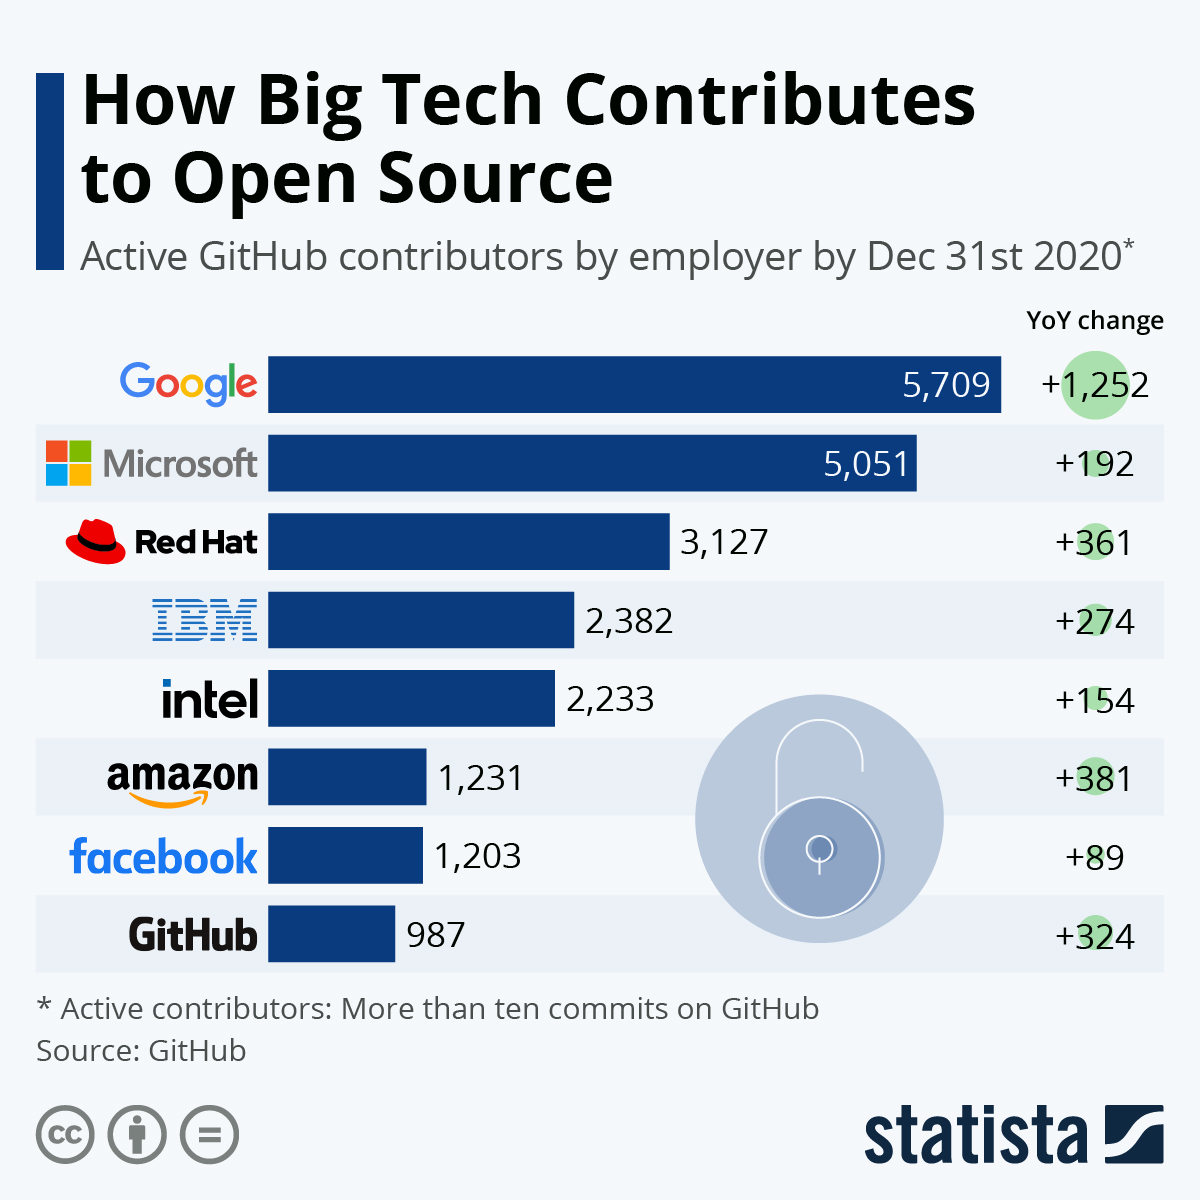
\includegraphics[width=11cm]{figs/bigtechcontributes.jpeg}
    \centering
    \caption{How How Big Tech Contributes to Open Source \cite{statista2021bigtechopensource}}
    \label{fig:bigtechcontributes}
\end{figure}


Current observations indicate a heightened workload for maintainers of open-source projects. Notably, the majority of contributions from external developers primarily consist of non-code based interactions such as comments, questions, issue reports, and pull request reviews. In contrast, developers employed by organizations continue to contribute code to their respective company's projects at a significantly higher rate than external contributors. The figure \ref{fig:percent_external_contributors} illustrates this trend, showing that most contributions are made by external developers, which did not belong to the organization that owns the repository.

Analysis of successful commercially-backed open-source projects on GitHub reveals that salaried developers employed by the companies behind these projects regularly contribute to them. This suggests that companies foster the most active and engaged communities when their developers actively participate as members of those communities, rather than simply releasing code under an open-source license.

\begin{figure}[ht]
    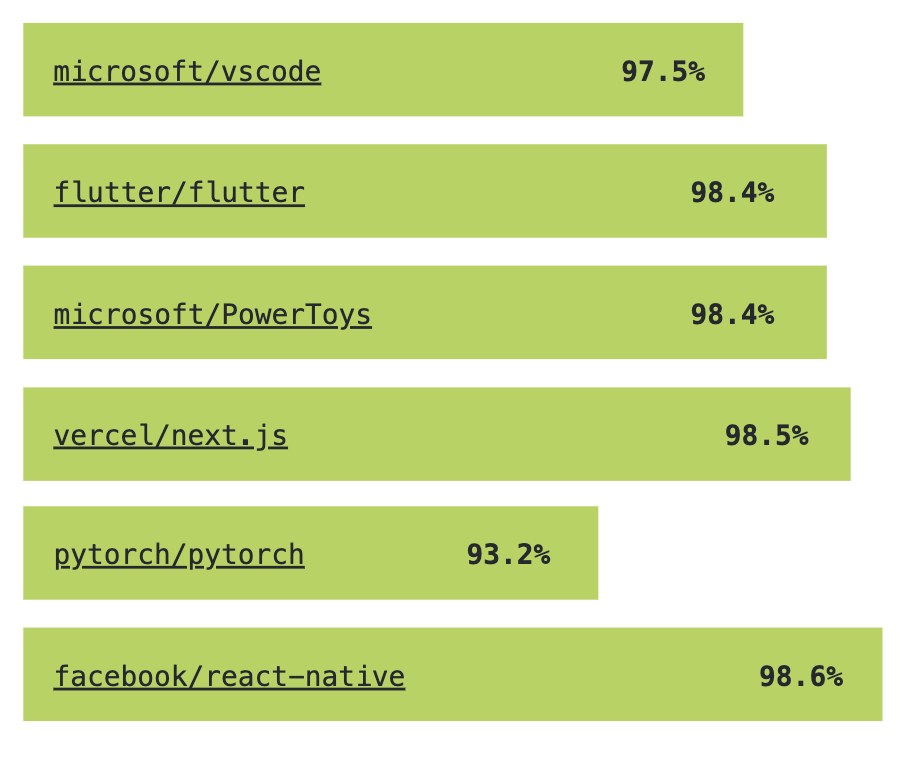
\includegraphics[width=10cm]{figs/percent_external_contributors.png}
    \centering
    \caption{Percentage of External Contributors}
    \label{fig:percent_external_contributors}
\end{figure}

The open-source movement's trajectory promises transformative impacts across industries, fueled by increasing collaboration, transparency, and knowledge sharing within its expanding community. This trajectory indicates the emergence of groundbreaking technologies, tools, and solutions that will serve the interests of both users and developers, underscoring the potential of open source to revolutionize sectors and drive innovation on a global scale.


\begin{figure}[ht]
    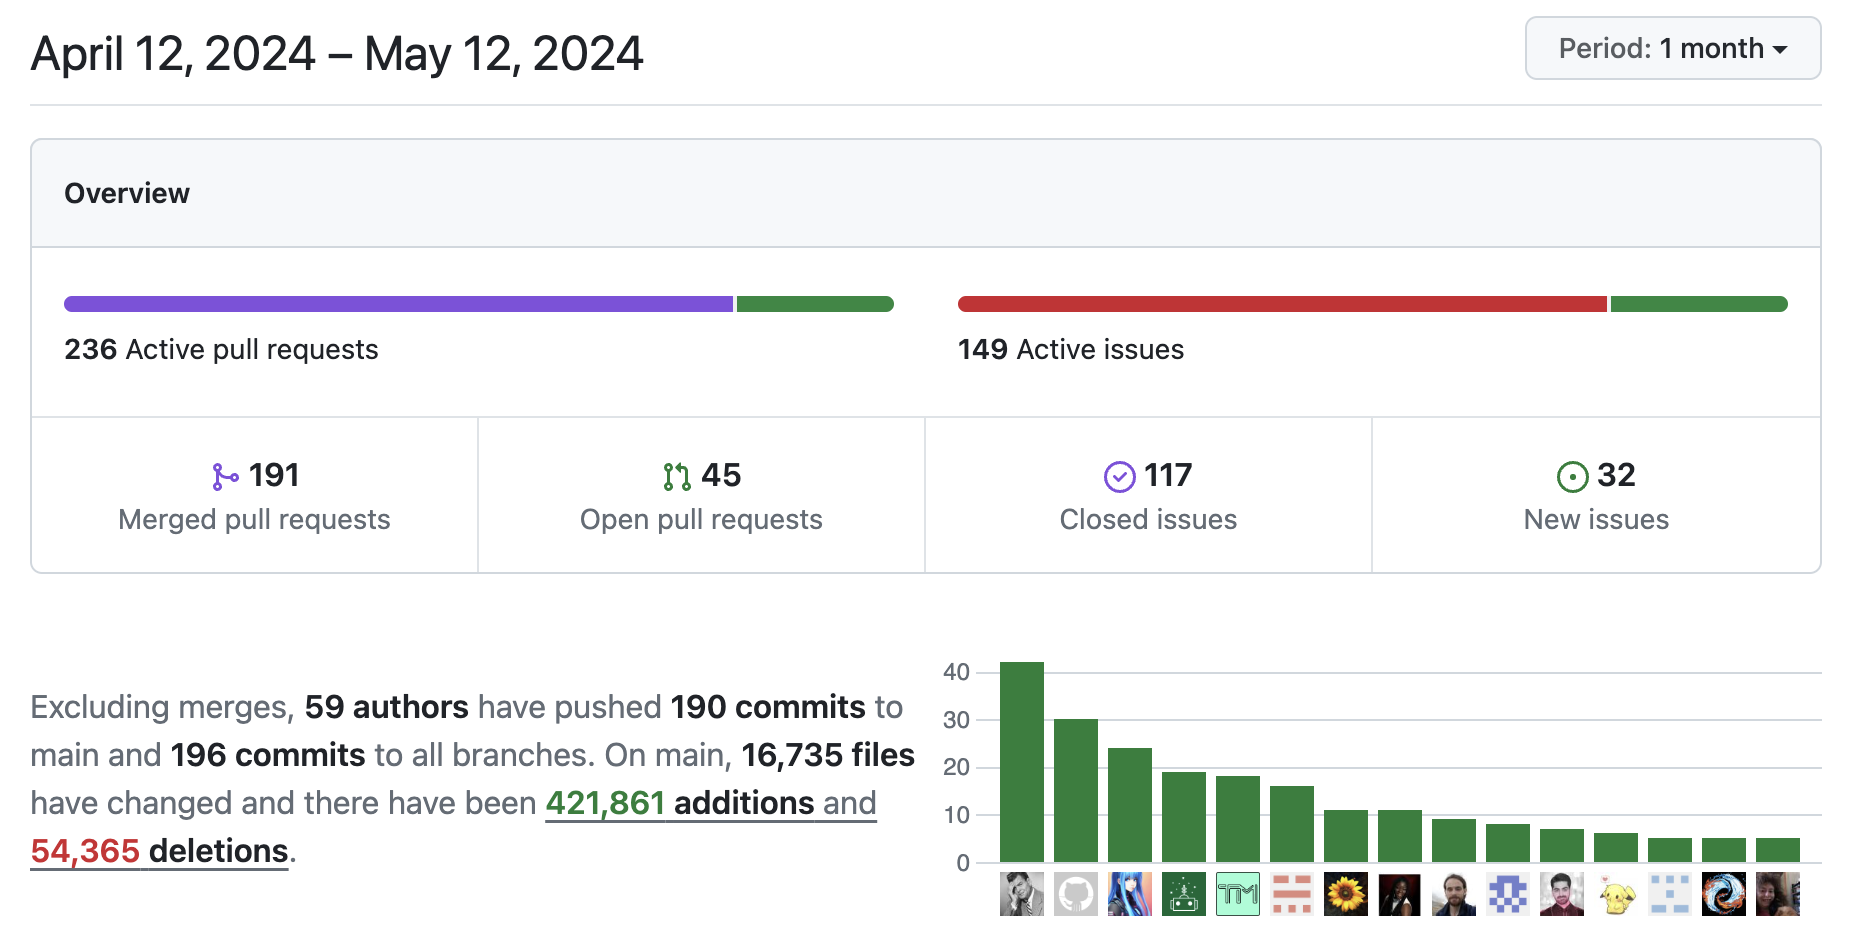
\includegraphics[width=1\linewidth]{figs/freecodecamp.png}
    \centering
    \caption{FreeCodeCamp's Open Source Contribution}
    \label{fig:freeCodeCamp}
\end{figure}





\clearpage  % This command will start the next section from the new page
